\documentclass[12pt]{article}
\usepackage[a4paper]{geometry}
%\userpackage[top=1 in, bottom=1.25 in, left=1.1 in, rigth=1.1 in] {geometry}
%\usepackage[paperwidth=17cm, paperheight=22.5cm, bottom=2.5cm, right=2.5cm]{geometry}
\usepackage[utf8]{inputenc}
%\usepackage[a4paper, top=2.5cm, bottom=2.5cm, left=2.2cm, right=2.2cm]
%{geometry}
%\usepackage[myheadings]{fullpage}
\usepackage{fancyhdr}
\usepackage{lastpage}
%\usepackage{float}
\usepackage{graphicx, wrapfig, subcaption, setspace, booktabs}
\usepackage{graphicx}
\usepackage[T1]{fontenc}
\usepackage[font=small, labelfont=bf]{caption}
%\usepackage{fourier}
\usepackage[protrusion=true, expansion=true]{microtype}
\usepackage[english]{babel}
\usepackage{sectsty}
\usepackage{url, lipsum}
\usepackage[T1]{fontenc}
\usepackage{icomma}
\usepackage{siunitx}
\usepackage{ragged2e}
\usepackage{amsmath}
\usepackage{comment}
\usepackage{enumerate}
%\usepackage{changepage}
\usepackage{anysize}




\newcommand{\HRule}[1]{\rule{\linewidth}{#1}}
\onehalfspacing
\setcounter{tocdepth}{5}
\setcounter{secnumdepth}{5}

%-------------------------------------------------------------------------------
% HEADER & FOOTER
%-------------------------------------------------------------------------------


\begin{comment}
-Udledninger
$$
\begin{aligned}
\end{aligned}
$$

-Opgavetekst
\begin{figure}[H]
\includegraphics[width=0.5\textwidth]{"path"}
\end{figure} 


-Opgave billede med tekst
\begin{figure}[H]
\caption{"Billedtekst"}
\includegraphics[width=0.5\textwidth]{"path"}
\end{figure} 

-Værdier
$\\
$


\end{comment}
\begin{document}

\begin{titlepage}

\title{ \normalsize 
		%\begin{figure}
        \begin{center}
        
\includegraphics[height=6cm]{Logo.jpg}
        \end{center}
       % \end{figure}
        \LARGE \textsc{\textbf{Universidad De Sonora}} \\ \bigskip
		\Large División de Ciencias Exactas y Naturales \\
        Licenciatura En Física \\ \bigskip
        \bigskip
        Física Computacional I
		\\ [0.1cm]  
		\HRule{2pt} \\
		\Large \textbf{{Actividad 7}} \\
        \textit{\textbf{"Álgebra Lineal con Python"}}
		\HRule{2pt} \\
		\normalsize \vspace*{0.001\baselineskip}}
        
\date{\bigskip \Large  \hspace*{\fill} Hermosillo, Sonora a marzo 07 de 2021}

        
\author{
		\Large\textbf{ Ismael Espinoza Arias} \\ \bigskip
        \\ \bigskip
       \Large Profesor Carlos Lizárraga Celaya}
       \end{titlepage}
       \maketitle
       
%-----------------------------------------------------------


\newpage
\pagestyle{plain}
\section{Introducción}
 En esta actividad trabajamos con el tema de álgebra lineal. Repasamos lo visto anteriormente en los cursos de álgebra lineal ahora implementando problemas computacionales con Python en la actividad de número 7. Hicimos uso de nuevas bibliotecas en Python, para poder realizar los ejercicios computacionales de nuestro nuevo tema para poder poner en práctica la teoría vista durante toda la semana. Es por eso que en esta sección trabajamos con los temas de matrices, determinantes, matrices cuadradas, el teorema de Caley-Hamilton, ecuaciones características, polinomios, resolución de sistema de ecuaciones, aplicaciones del Gauss-Jordan y eliminación Gaussiana, soluciones entre otras funciones elementales del álgebra lineal. 


%-----------------------------------------------------------


\section{Comentarios}

Para poder desarrollar las actividades en esta sección, debimos ver la teoría semanal impartida por el docente, con ella y con la resolución de unos ejercicios fue como desarrollamos las habilidades requeridas en esta actividad. Primero encontramos el uso de las nuevas bibliotecas que en nuestro caso son: Scipy.linalg, Numpy.linalg  y el uso de unas bibliotecas que ya estábamos previamente usando pero que resultan muy efectivas, Numpy y Matplotlib.pyplot.\\
Después nos encontramos con los ejercicios compuatcionales, como lo son la definición de matrices con Python, la demostración del teorema de Caley-Hamilton, la resolución de un sistema de ecuaciones por el método de eliminación gaussiana, encontrar los eigenvectores y los eigenvalores de una matriz, realizar una interpolación polinómica y por último una regresión lineal de las temperaturas ya antes utilizadas en el curso.\\
Una de las herramientas matemáticas más utilizadas en machine learning y data mining es el Álgebra lineal, por lo tanto, si queremos incursionar en el fascinante mundo del aprendizaje automático y el análisis de datos es importante reforzar los conceptos que forman parte de sus cimientos.\\
Como ya sabemos el Álgebra lineal es una rama de las matemáticas que es sumamente utilizada en el estudio de una gran variedad de ciencias, como ser, ingeniería, finanzas, investigación operativa, entre otras. Es una extensión del álgebra que aprendemos en la escuela secundaria, hacia un mayor número de dimensiones; en lugar de trabajar con incógnitas a nivel de escalares comenzamos a trabajar con matrices y vectores.\\



%-----------------------------------------------------------


\section{Desarrollo de la actividad}

Empezamos importando nuestras bibliotecas:

    \begin{center}
	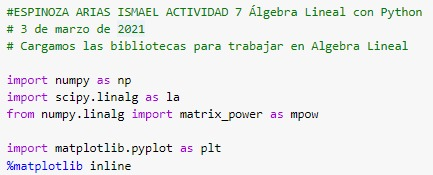
\includegraphics[height=6cm]{Bibliotecas.jpeg}\\
    \end{center}
    
Procediamos a definir las matrices con las que hibamos a operar:

    \begin{center}
	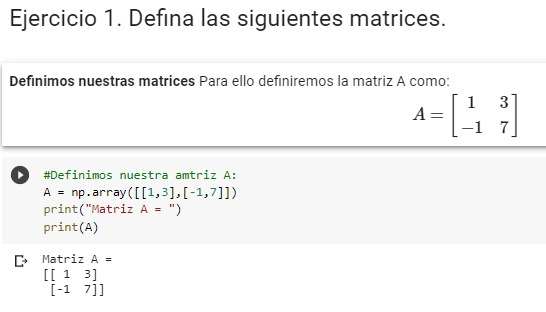
\includegraphics[height=9cm]{E1.jpeg}\\
    \end{center}

Después solamente, definimos de la misma forma cada matriz y con estas fuimos operando.\\
En el ejercicio 2, nos encontramos con la demostración del teorema de Caley-Hamilton, donde tenemos lo siguiente:

    \begin{center}
	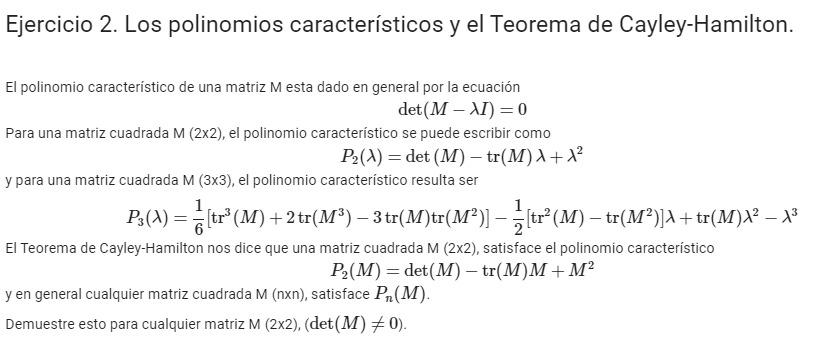
\includegraphics[height=7cm]{E2.jpeg}\\
    \end{center}
    
Para la demostración de este teorema, lo que hicimos fue hacerlo de forma general, y después con un ejemplo en especifico para confirmar que se cumple apara cualquier matriz cuadrada con determinante distinto de 0.\\

    \begin{center}
	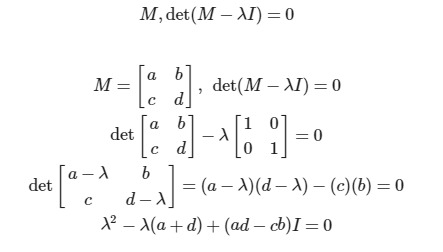
\includegraphics[height=8cm]{E.2.1.jpeg}\\
    \end{center}

    \begin{center}
	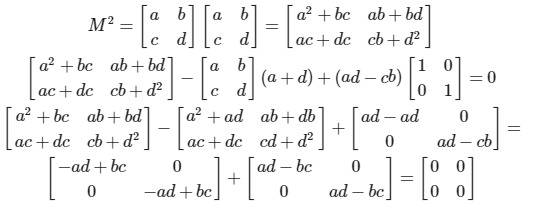
\includegraphics[height=6.5cm]{E2.2.jpeg}\\
    \end{center}
    
Con esta demostración, ya solo nos queda el ejemplo de como aplicarlo en un caso específico, en este caso la matriz M.\\

    \begin{center}
	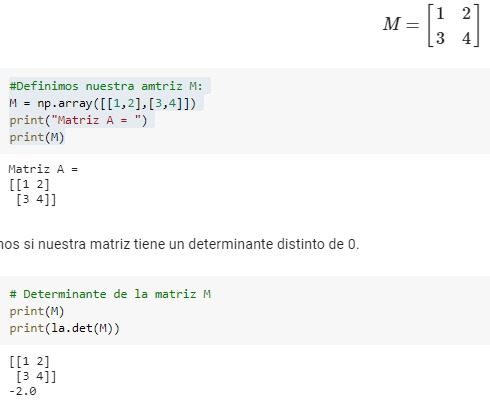
\includegraphics[height=13cm]{E2.3.jpeg}\\
    \end{center}

    \begin{center}
	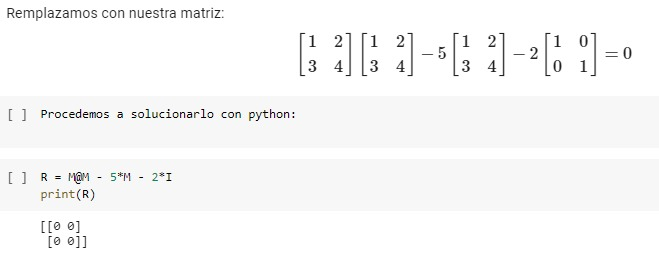
\includegraphics[height=7cm]{E2.5.jpeg}\\
    \end{center}
\textbf{Por lo tanto queda demostrado el teorema anterior.}\\

Con la siguiente ejercicio solucionamos un sistema de ecuaciones por medio del método de eliminación Gaussiana.

    \begin{center}
	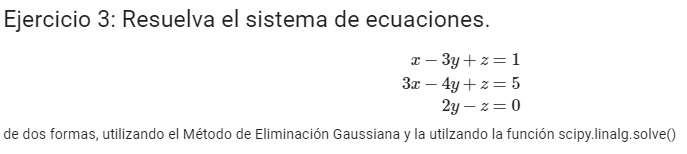
\includegraphics[height=3.8cm]{E3.jpeg}\\
    \end{center}
    
Definiremos 3 funciones que nos ayudaran a resolver este sistema:

    \begin{center}
	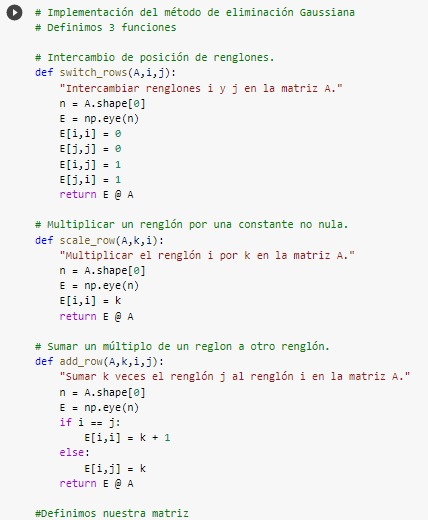
\includegraphics[height=21cm]{E3.1.jpeg}\\
    \end{center}
    
    \begin{center}
	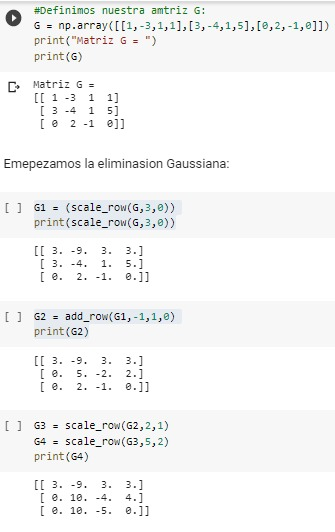
\includegraphics[height=21cm]{E3.2.jpeg}\\
    \end{center}
    
Lllegamos al final, al siguiente resulatdo:

    \begin{center}
	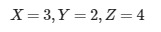
\includegraphics[height=1cm]{E3.3.jpeg}\\
    \end{center}

Pasamos al sigueinte ejercicio.

    \begin{center}
    	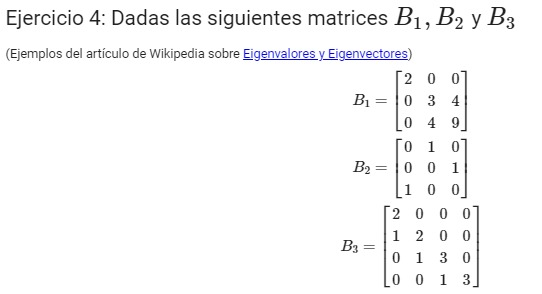
\includegraphics[height=9cm]{E4.jpeg}\\
    \end{center}
 Aquí, haremos cosas similares como en los ejercicios anteriores, donde vamos a definir nuestras amtrices y procedemos a usar las fórmulas de nuestars bibliotecas para consegiuir por pedido.
 
     \begin{center}
	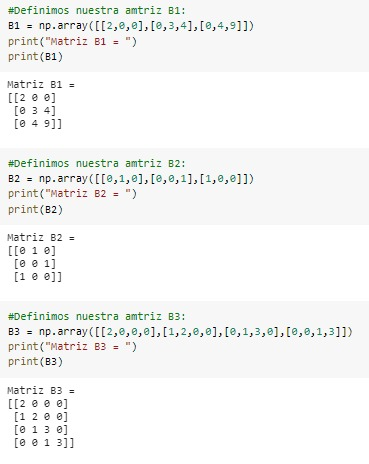
\includegraphics[height=18cm]{E4.1.jpeg}\\
    \end{center}
    
    \begin{center}
	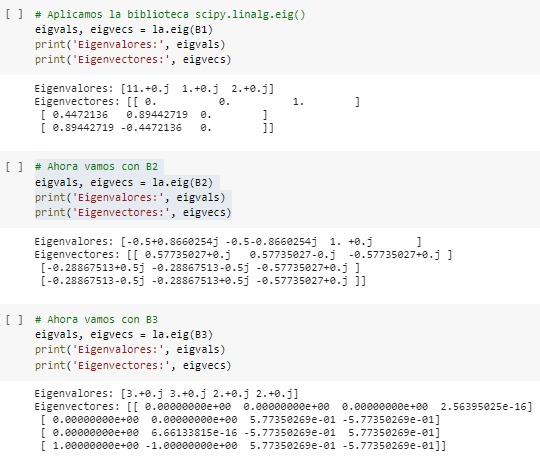
\includegraphics[height=14cm]{E4.3.jpeg}\\
    \end{center}
    
Ahora pasamos al ejercicio 5.

    \begin{center}
	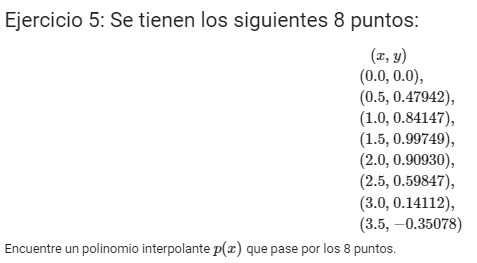
\includegraphics[height=7cm]{E5.jpeg}\\
    \end{center}
    
Graficamos nuestros datos y después vemos las gráficas:

    \begin{center}
	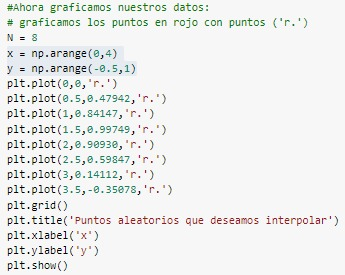
\includegraphics[height=13cm]{E5.1.jpeg}\\
    \end{center}
    
    \begin{center}
	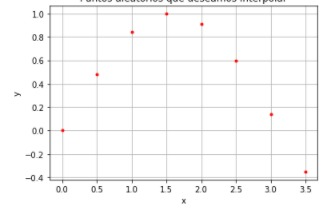
\includegraphics[height=10cm]{E5.3.jpeg}\\
    \end{center}

Después de la interpolación, llegamos al siguiente gráfico:

    \begin{center}
	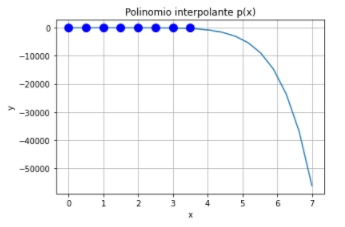
\includegraphics[height=10cm]{5.4.jpeg}\\
    \end{center}
    
Llegamos al último ejercicio de la actividad 7, que consiste en hacer una regresión lineal con nuestros datos de las temepraturas anteriores.

    \begin{center}
	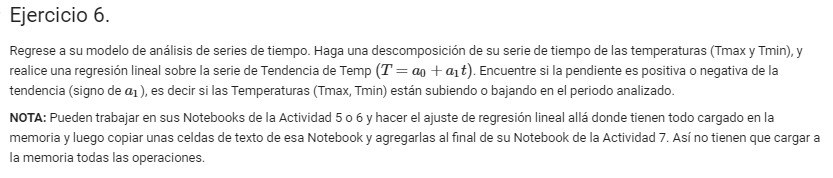
\includegraphics[height=3.5cm]{E6.jpeg}\\
    \end{center}
    
    \begin{center}
	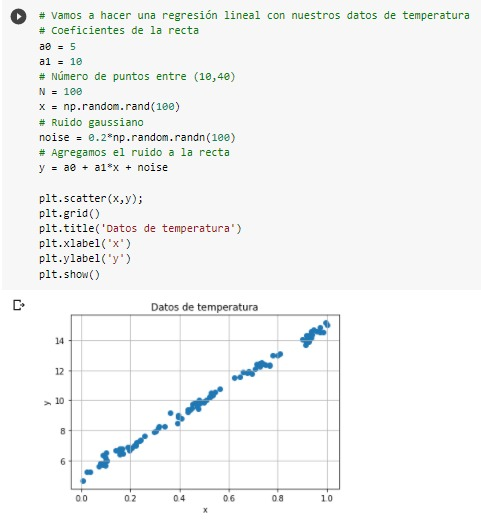
\includegraphics[height=18cm]{E6.1.jpeg}\\
    \end{center}
    
    Obtuvimos las siguientes gráficas:
    
    \begin{center}
	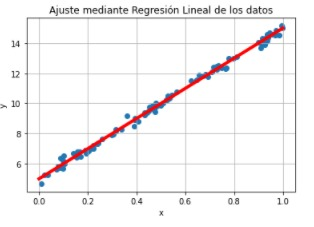
\includegraphics[height=8cm]{E6.2.jpeg}\\
    \end{center}
 
    \begin{center}
	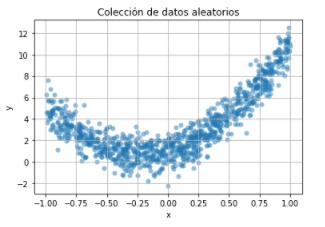
\includegraphics[height=8cm]{E6.3.jpeg}\\
    \end{center}
    
    \begin{center}
	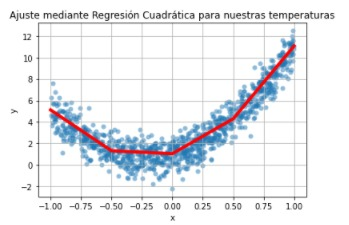
\includegraphics[height=8cm]{E6.4.jpeg}\\
    \end{center}
    
\textbf{Concluimos las actividades de esta semana.}
    

%-----------------------------------------------------------


\section{Conclusión}

Como conclusión, podemos ver que es fundamental el álgebra lineal en la física computacional, ya que con esta podemos modelar muchas situaciones de la vida real y poder jugar con los datos de formas en las que podamos usar los datos y sus predicciones a nuestro favor. Es por eso que haber realizado esta actividad me gusto mucho por que se relaciona con lo que me quiero de dedicar terminando la universidad, a al ciencia de datos, a lo que se relaciona todo esto de la estadística, el álgebra lineal y la física computacional. 


%-----------------------------------------------------------


\section{Apéndice}
\begin{enumerate}
\item \textbf{¿Qué te pareció el tema de Análisis de Series de Datos?}\\
\textit{Me pareció muy bien la actividad, ya que como en un futuro me gustaría enfocarme en la ciencia de datos, esta actividad se relaciona mucho con ello, es por eso le pongo mucha atención y hago todo lo posible por aprender acerca de estos temas.}

\item \textbf{¿Cómo estuvo el reto?}\\
\textit{Estuvo algo difícil, ya que no pude compilar en ciertas ocasiones y fue muy difícil encontrar el error, pero al final todo salió bien y me gusto la actividad. Si tuviera que agregar algo, es que no tenía un concocimiento sólido en el álgebra lineal, ya que considero que el docente que me impartio la materia no lo hizo de la mejor formar posible, por ser principios de la pandemia.}

\item \textbf{¿ ¿Qué se te dificultó más??} \\
\textit{El repasar los temas de álgebra lineal y encontrar algunas cosas que no tenía tan sólida mi formación.}

\item \textbf{¿Qué te aburrió?}\\
\textit{Nada en concreto, todo creo que fue de suma importancia y que en todo momento todo fue muy activo y dinámico.}

\item \textbf{¿Qué recomendarías para mejorar la primera Actividad?? }\\
\textit{Nada en especial, ya que me gusto mucho como esta implementada esta actividad, pero si vieran un poco más a fondo la ciencia de datos, sería mejor para mí.}

\item \textbf{¿Que grado de complejidad le asignarías a esta Actividad? (Bajo, Intermedio, Avanzado)} \\
\textit{Le asignaría un mediano, porque todavía no consideró que la actividad sea demasiado difícil como para que se vuelva intensivo el ejercicio, pero no es lo más fácil del mundo ya que debemos de mover los datos y ajustarlos a nuestro modelo, y prácticamente llevar el álgebra lineal al medio computacional.}

%-----------------------------------------------------------


\section{Bibliografía}
\begin{enumerate}
\item \textit{Linear Algebra with SciPy - Mathematical Python. (s. f.). Mathematical Python. Recuperado 7 de marzo de 2021, de https://www.math.ubc.ca/\%7Epwalls/math-python/linear-algebra/linear-algebra-scipy/.}

\item \textit{Solving Linear Systems - Mathematical Python. (s. f.). Mathematical Python. Recuperado 7 de marzo de 2021, de https://www.math.ubc.ca/\%7Epwalls/math-python/linear-algebra/solving-linear-systems/.}

\item \textit{Eigenvalues and Eigenvectors - Mathematical Python. (s. f.). Mathematical Python. Recuperado 7 de marzo de 2021, de https://www.math.ubc.ca/\%7Epwalls-- /math-python/linearalgebra/eigenvalues-eigenvectors/.}

\item \textit{Applications - Mathematical Python. (s. f.). Mathematical Python. Recuperado 7 de marzo de 2021, de https://www.math.ubc.ca/\%7Epwalls/math-python/linear-algebra/applications/.}

\item \textit{Briega, L. R. E. (2015, 14 junio). Algebra Lineal con Python. Matemáticas, análisis de datos y python. https://relopezbriega.github.io/blog/2015/06/14/algebra-lineal-con-python/}
   
 \end{enumerate}
\end{enumerate}


%-----------------------------------------------------------

\end{document}